\chapter{Classical Oscillator}
We begin our investigation of a cOM apparatus by first modeling a classical mechanical oscillator. Our approach is to transform operators into conventional classical functions, and we do so using two different methods. First, the standard cQED apparatus is mechanically coupled to a harmonic oscillator following a sine function. Second, the oscillator is placed in a thermal state and undergoes Brownian motion using a pseudorandom number generator. Plots of mean photon number of the cavity mode and mean atomic excitation number over time provide baseline dynamics that can be compared when the oscillator is written using operator formalism.

\section{Harmonic Oscillator}
For a sinusoidal oscillator, we consider the necessary modifications to the Hamiltonian of \eqref{eq2.107}. Appealing to simplicity, we consider a driving field resonant with the cavity mode and atomic transition, such that the $\Delta$ term vanishes. Because the $\hbar\omega_M \, \bdag b$ term reflects an internal energy of the mechanical oscillator, we may, in the classical picture, conceive of it as an energy offset to the Hamiltonian; this could be subtracted away in an experimental apparatus and as such we disregard the $\bdag b$ term as well. Lastly, because we take the oscillator to be at zero temperature, the $\kappa_M$ term is omitted. This leaves us with the driving term, two coupling terms, and two modes of dissipation,
%
\be \begin{split} H'_{\text{harmonic}} &= \hbar Y \left( a + \adag \right) + \hbar g \left( a\splus + \adag\sminus \right) + \hbar g_M \, \adag a \left( b + \bdag \right) \\
&\qquad - i\hbar\kappa \, \adag a - i\hbar\frac{\gamma}{2} \, \splus\sminus, \label{eq3.1} \end{split} \ee
%
where the prime denotes that we have yet to convert the position operator $\hat{x}$ of \eqref{eq2.105} to a classical function. For the sinusoidal case, the end mirror of the cavity oscillates with frequency $\omega_M$ such that \eqref{eq3.1} is now
%
\be \begin{split} H_{\text{harmonic}} &= \hbar Y \left( a + \adag \right) + \hbar g \left( a\splus + \adag\sminus \right) + \hbar g_M \, \adag a \, \sin(\omega_M t) \\
&\qquad - i\hbar\kappa \, \adag a - i\hbar\frac{\gamma}{2} \, \splus\sminus. \label{eq3.2} \end{split} \ee
%
Using QuTiP and the \texttt{odesolve} function, the Schr\"{o}dinger equation is numerically evaluated using Hamiltonian \eqref{eq3.2} to determine the expectation values $\langle \adag a \rangle$ and $\langle \splus\sminus \rangle$, whose traces are shown below.
%
\begin{figure}[htb]
\begin{center}
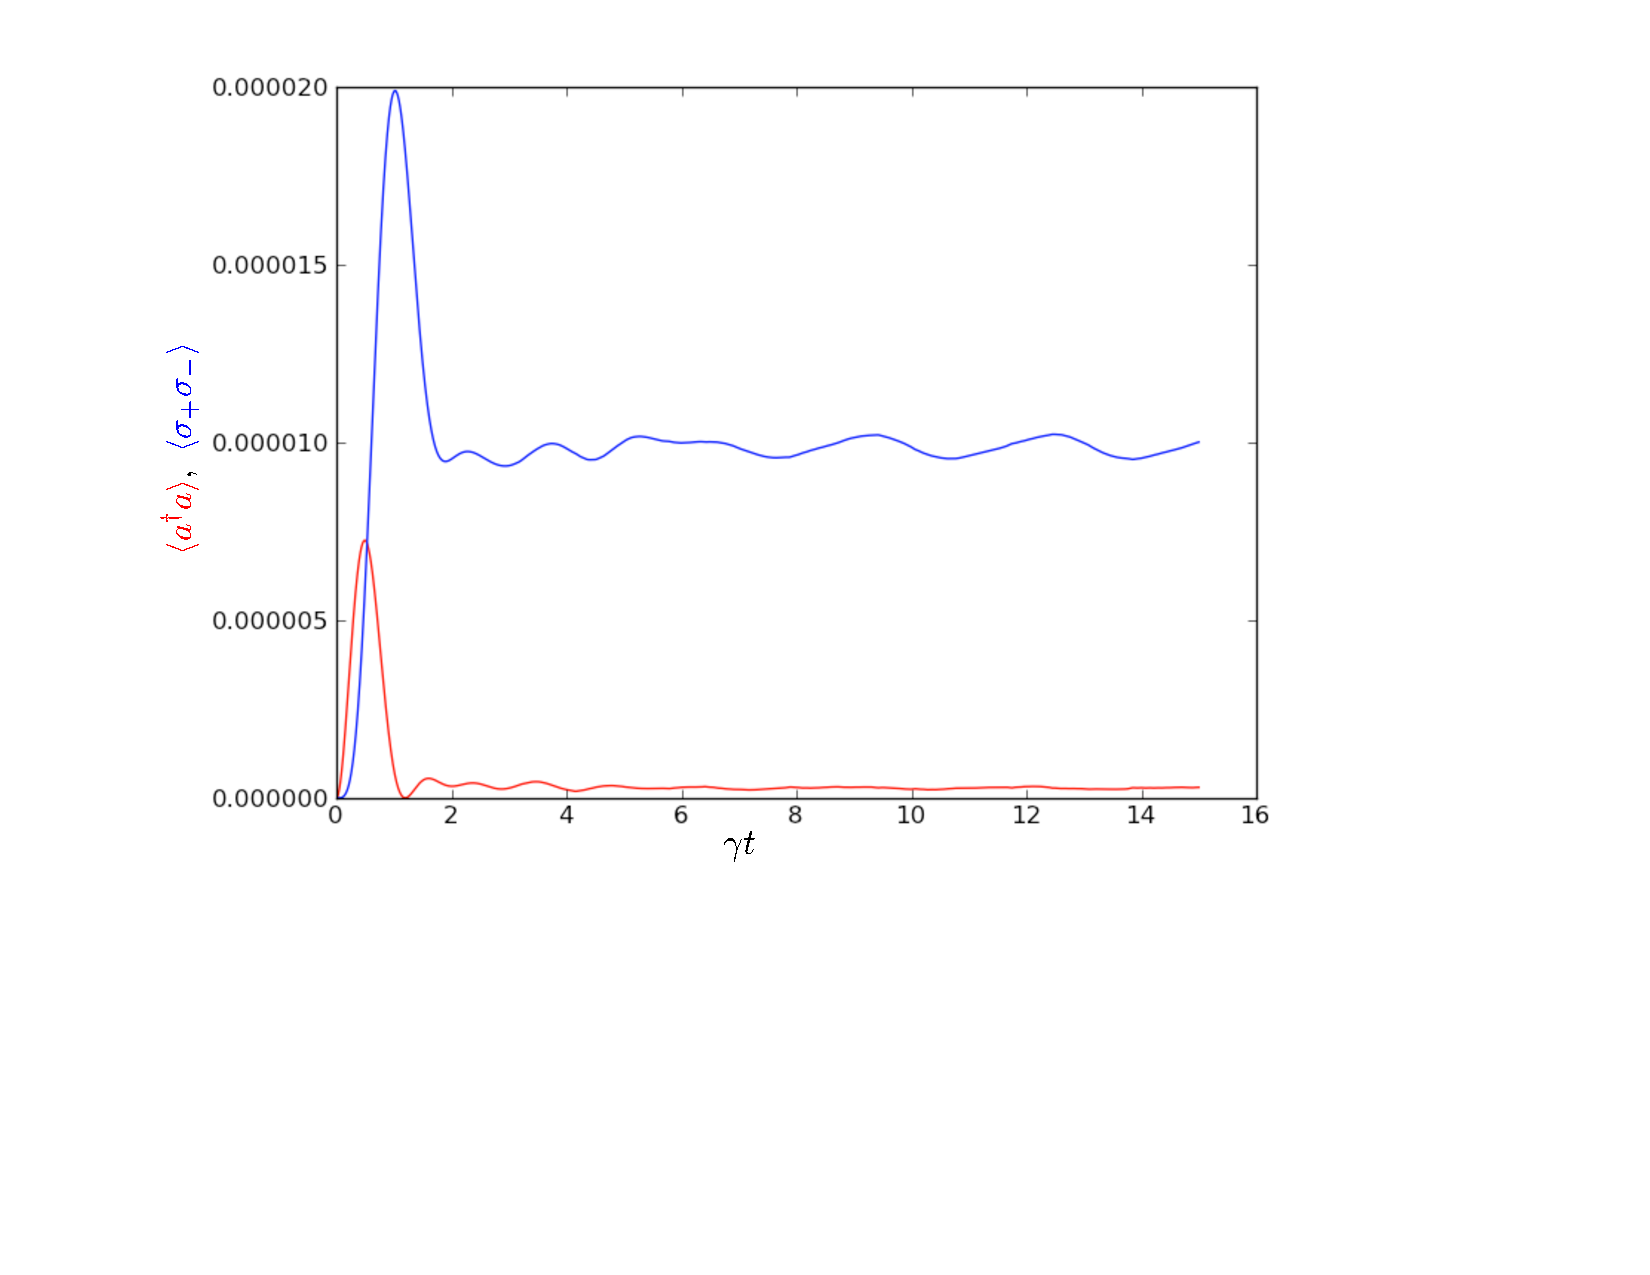
\includegraphics[width=0.85\textwidth]{Figures/3HarmonicPlots}
\caption[A plot of the expectation values $\langle \adag a \rangle$ and $\langle \splus\sminus \rangle$ for the harmonic oscillator]{\small{A plot of the expectation values $\langle \adag a \rangle$ and $\langle \splus\sminus \rangle$. The two quantities are calculated over fifteen spontaneous emission lifetimes; red denotes $\langle \adag a \rangle$ and blue denotes $\langle \splus\sminus \rangle$. The relevant parameters are $\gamma = \kappa = \omega_M = 1$, $Y/\gamma = 0.01$, $g/\gamma = 3$, and $g_M/\gamma = 2$.}}
\label{fig3Harmonic}
\end{center}
\end{figure}
%
In order to emphasize our consideration of weak driving, we will, in all cases, allow at most two excitations in the atom-cavity subsystem. Before we comment upon Fig.~\ref{fig3Harmonic}, we proceed to consider the next type of classical mechanical oscillator and its analogous plot.

\section{Thermal Oscillator}
In this second approach to the classical picture, we consider the situation where the oscillating end mirror is placed in a thermal state, i.e. the mirror undergoes Brownian motion. We will incorporate the same approximations as in Section~3.1, such that the preliminary Hamiltonian will be identical to \eqref{eq3.1}, or $H'_{\text{thermal}} = H'_{\text{harmonic}}$. To transform to a classical term as in \eqref{eq3.2}, we write
%
\be \begin{split} H_{\text{thermal}} &= \hbar Y \left( a + \adag \right) + \hbar g \left( a\splus + \adag\sminus \right) + \hbar g_M \, \adag a \, \xi \\
&\qquad - i\hbar\kappa \, \adag a - i\hbar\frac{\gamma}{2} \, \splus\sminus, \label{eq3.3} \end{split} \ee
%
where $\xi$ is a pseudorandom number generated by QuTiP in the range $\xi \in$ (0, 1) chosen once for each trajectory. Again as in Section~3.1, we calculated expectation values for the cavity mode and two-level atom over time. These traces are shown below.
%
\begin{figure}[htb]
\begin{center}
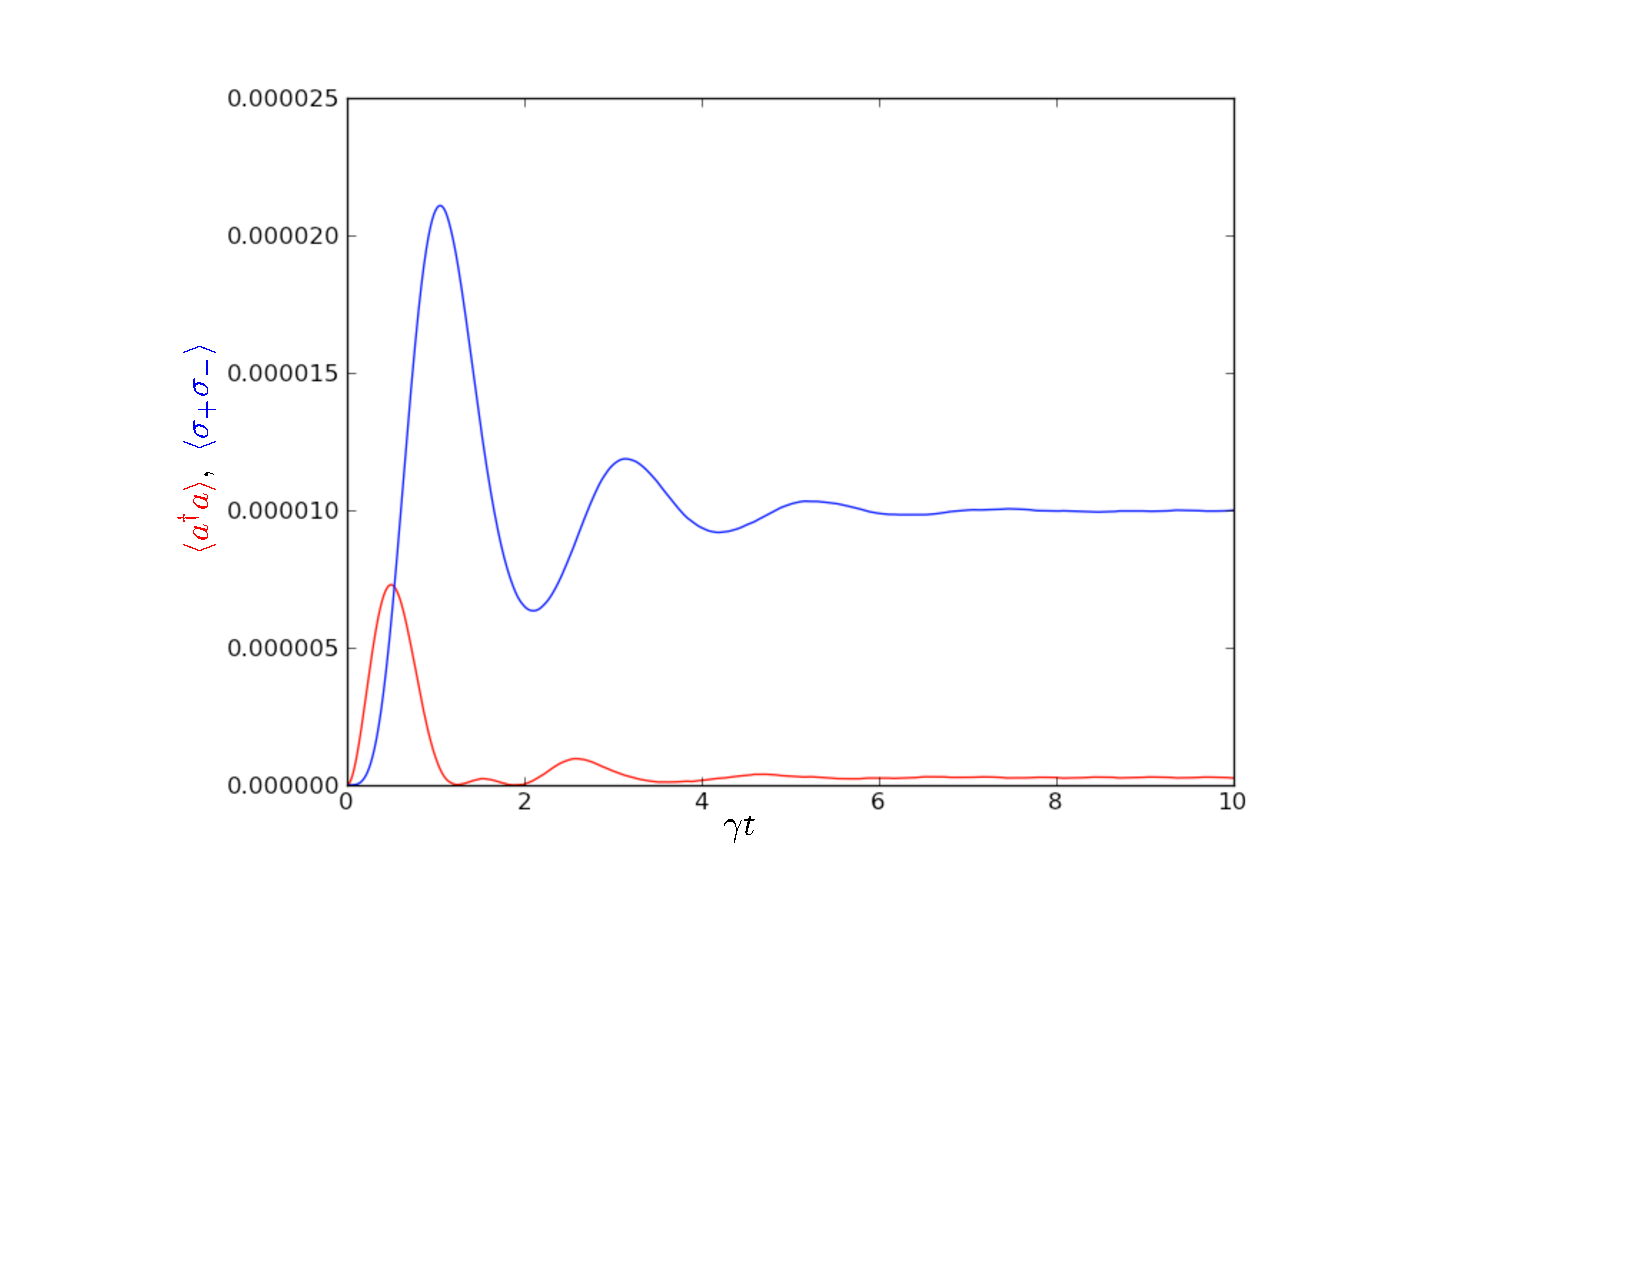
\includegraphics[width=0.85\textwidth]{Figures/4ThermalPlots}
\caption[A plot of the expectation values $\langle \adag a \rangle$ and $\langle \splus\sminus \rangle$ for the thermal oscillator]{\small{A plot of the expectation values $\langle \adag a \rangle$ and $\langle \splus\sminus \rangle$. The two quantities are calculated over ten spontaneous emission lifetimes; red denotes $\langle \adag a \rangle$ and blue denotes $\langle \splus\sminus \rangle$. The relevant parameters are identical to Fig.~\ref{fig3Harmonic} with the exception of $\omega_M$, which was not referenced in this calculation.}}
\label{fig4Thermal}
\end{center}
\end{figure}

We first consider the steady-state results of both figures. For the harmonic oscillator, the respective lengths of time for $\langle \adag a \rangle$ and $\langle \splus\sminus \rangle$ to settle are approximately $7\tau_0$ and $9\tau_0$, while in the thermal oscillator we see $6\tau_0$ and $8\tau_0$; we have introduced the spontaneous emission lifetime $\tau_0 = 1/\gamma$. Another important feature is that both plots lie in the same order of magnitude, we see $\langle \adag a \rangle$ and $\langle \splus\sminus \rangle \sim 10^{-5}$. It follows that Figs.~\ref{fig3Harmonic} and \ref{fig4Thermal} are similar in range and appearance, as their respective Hamiltonians \eqref{eq3.2} and \eqref{eq3.3} differ only by a constant factor in the $g_M$ coupling term. While \eqref{eq3.2} sees the coupling oscillate between $\pm 1$, the thermal oscillator \eqref{eq3.3} produces a constant coupling whose magnitude is dictated by $\xi$.

We have discovered baseline behavior for the mechanical oscillator in both the harmonic and thermal cases, where an initial excitation due to driving of the cavity mode pushes the mean cavity photon number and atomic excitation number settles to a steady-state value after fewer than ten spontaneous emission lifetimes of the atom. It would also prove useful to discuss experimental values for the various parameters of the system in order to provide some numerical perspective. The spontaneous emission rate is typically in the microwave region, on the order of 1-10 GHz, which also sets the scale for the cavity decay rate. Most versions of an experimental optomechanical apparatus realize mechanical frequencies $\omega_M$ on the order of 1-10 MHz \cite{arcizet2006, kippenberg2005, kimble2009}, but we follow the lead of \cite{thompson2007} in using mechanical frequencies on the order of $\gamma$ and $\kappa$. With these numbers in mind, we are now ready to proceed to a full quantum treatment of the cOM system.